%%
\chapter{Generating components for runtime model handling}
%%

faIn this chapter, we show, how we generate the \cpp{} components capable of creating and maintaining the model representing the system. 
The input for the generation is the EMF Ecore metamodel of the system, so it must be available at this step of the system developement. 


%%%%
%%%%
%%%%
\section{Source code structure}
%%%%
%%%%
%%%%

The domain model consists of 
\begin{itemize}
	\item packages (EPackage)
	\item classes (EClass) 
	\item and enumerations (EEnum).
\end{itemize}

From an EPackage, we generate a folder; Every source file originated from an elements from the package will be generated in that folder. 
We generate sources from each class and enumeration of the package, also we generate other artifacts for the package: helper classes and model handling utilities.


\section{Mapping EClasses to \protect\cpptt{} classes}


\begin{figure}
	\begin{center}
		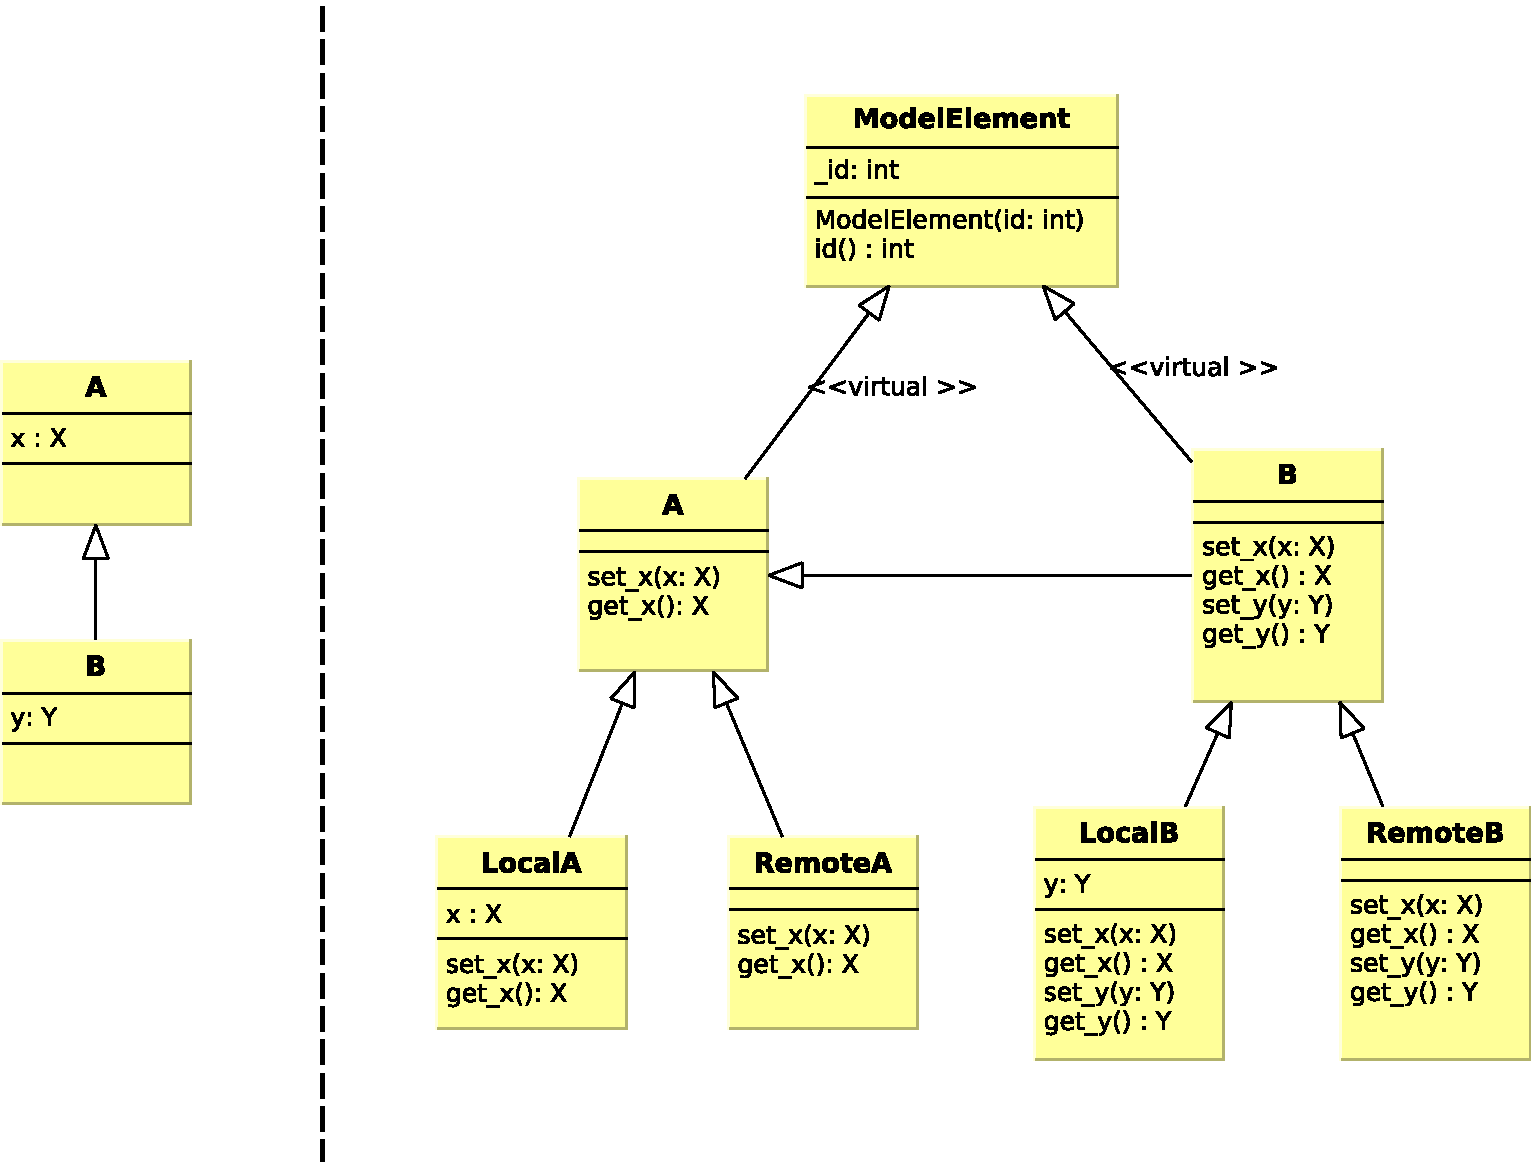
\includegraphics[width=\textwidth]{figures/eclass-to-cpp.pdf}
		\caption{Mapping of two EClasses, one inherited from the other (Left: EClasses, right: \protect\cpp{} classes) }
		\label{fig:eclass-to-cpp}
	\end{center}
\end{figure}


The EClasses of the metamodel are mapped to various \cpp{} classes, as depicted on \mbox{\autoref{fig:eclass-to-cpp}}.
From each EClass we generate three \cpp{} classes:

\begin{itemize}
	\item An interface (abstract class with only pure virtual methods in \cpp{})
	\item A local class
	\item A remote class
\end{itemize}


The interface provides access to an instance of the EClass.
The local class implements the interface. It stores the attributes and references of the instances allocated to the local computing unit, and made them accessible by the methods of the implemented interface.
The remote class implements the interface, but are only used to substitute remote objects in references to them; 
Accessing its variables are not possible, because they are stored in another node. 

\section{Mapping EEnums to \protect\cpptt{} enumerations }

For each EEnum, a C++ enum class with the same name is generated. For each EEnumLiteral a C++ enumeration literal is added in the generated code as it is depicted in \autoref{fig:eenum-to-cpp}.

\begin{figure}[H]
	\begin{center}
		
		\begin{minipage}[c]{\textwidth}
		\begin{minipage}[r]{0.52\textwidth}
			\hfill
			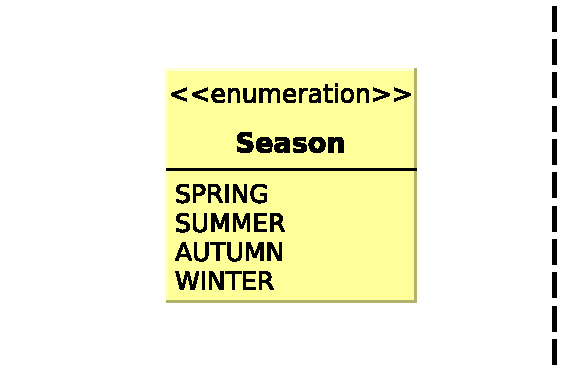
\includegraphics[width=0.735\textwidth]{figures/eenum-to-cpp.pdf}
		\end{minipage}
			\hspace{0.05\textwidth}
		\begin{minipage}[c]{0.25\textwidth}
\begin{lstlisting}[language=C++]
namespace Package{
	
	enum class Season{
		SPRING = 0,
		SUMMER = 1,
		AUTUMN = 2,
		WINTER = 3
	};

}
\end{lstlisting}			
		\end{minipage}
		\end{minipage}
		\caption{Mapping of an enumeration to \protect\cpp{} enum class }
		\label{fig:eenum-to-cpp}
	\end{center}
\end{figure}


The framework also generates an EnumHelper class and specializes it for generated enumerations. Such helper classes are necessery in order to  parse enumerations from string, or convert them to string, as these are not supported by \cpp{}. Eg.\ for the enumeration in \autoref{fig:eenum-to-cpp} the framework generates the following template specialization:

\begin{minipage}{\textwidth}
\begin{lstlisting}[language=C++]
template<>
struct EnumHelper< ::Package::Season> {
	static const char* ToString(::Package::Season x)
	{
		switch (x)
		{
			case ::Package::Season::SPRING: return "SPRING";
			case ::Package::Season::SUMMER: return "SUMMER";
			case ::Package::Season::AUTUMN: return "AUTUMN";
			case ::Package::Season::WINTER: return "WINTER";
			
			default:
				throw "Invalid enumeration value";
		}
	}
	
	static ::Package::Season ParseFromString(const std::string& str)
	{
		if(str == "SPRING")
			return ::Package::Season::SPRING;
		if(str == "SUMMER")
			return ::Package::Season::SUMMER;
		if(str == "AUTUMN")
			return ::Package::Season::AUTUMN;
		if(str == "WINTER")
			return ::Package::Season::WINTER;
		
		throw "EnumHelper ParseFromString method: input string cannot be interpreted.";
	}
};
\end{lstlisting}
\end{minipage}


\section{ Generating ModelRoot class }

A class called \texttt{ModelRoot} is also generated.
The purpose of \texttt{ModelRoot} is to handle the whole model of the system: 
It contains the instances of the classes and it keeps track of the objects by identifier.
It also provides a method to read in initial models from a json file.
The \texttt{ModelRoot} class is also the connection point between the monitoring components and the model.

\section{ Other sources }

For each package the framework generates
\begin{itemize}
	\item a header file containing forward declarations for each generated classes
	\item a header file including all the full declaration of classes
\end{itemize} 

